\documentclass[twocolumn, 9pt,fleqn]{jsproceedings}

\interfootnotelinepenalty=10000

\title{Mobile Robot Path Drift Estimation using Visual Streams}

\author{Helio Perroni Filho (Doctorate Course, 1st year)\authorrefmark{1}}

\affiliation{Intelligent Robotics Laboratory, OHYA's group}

\abstract{
This article describes a new approach for visual navigation under the teach-replay paradigm. Dubbed Differential Visual Stream, or DiVS for short, it only requires a single front-mounted monocular camera for input; it dispenses with any form of calibration, including calibration for intrinsic camera parameters (e.g. lens distortion). The method relies on the calculation of difference images to measure the rate of change over the the visual input stream; this information is used to characterize both the landscape in front of the robot and its position within the surrounding environment. Experiments show DiVS is robust to lighting variations and changes to the visual composition of the landscape, and works well both indoors and outdoors. The article concludes with a discussion on further research.
}

\keywords{Image Processing, Machine Learning, Navigation}

\begin{document}
\thispagestyle{myheadings}
\markright{2014年度 第1回 山彦シンポジウム [2014/8/7--8/9 山中共同研修所]}
\maketitle

\authorreftext{1}{Graduate School of Systems and Information Engineering,\\ University of Tsukuba}

\section{Introduction}

Autonomous navigation is a central topic in mobile robotics, with a range of useful applications~\cite{BON02,ARK90}. In particular, given the advantages of cameras over other sensors~\cite{BON02,DAV07}, robust vision-based navigation has long been considered an important research goal. Methods proposed over the years can be roughly divided into \textit{map-based} and \textit{mapless}, according to whether they depend on globally consistent world representations~\cite{BON02}.

Simultaneous Localization and Mapping (SLAM) is a popular map-based approach. Initially supported mainly by range sensors such as laser and ultrasound, recent advances and wider hardware availability have increased the number of such systems that employ cameras as navigation sensors~\cite{DAV07,CUM08}. Unfortunately, the need to keep an accurate map, and precisely track the robot's pose within it, have always placed an upper bound on the geographic range a SLAM system can reliably navigate.

The complexity and limitations of map-based navigation systems have motivated work in mapless methods. In particular, \textit{appearance-based} navigation represents the world as sequences of ``snapshots'' collected along a route, which are later matched to live sensory input in order to estimate the robot's present location. Its development has been partly inspired by studies on insects such as bees and ants, whose homing skills do not seem to be based on detailed geometrical representations~\cite{VAR05}. ``Teach-replay'' is the typical scenario for appearance-based navigation: a robot is first guided through an environment (the teaching phase), and must then autonomously retrace the original path (the replay phase)~\cite{BUR01}. A wide variety of vision-based solutions have been applied to this problem~\cite{VAR05,BUR01,OYA96,MAT96,LAM00,CHE06} over the years. However, experimental systems are often restricted to environments with limited lighting variation, devoid of changes to landscape composition or moving elements such as people and other machines~\cite{KIM08}. This is understandable, since visual recognition of objects and places, upon which many visual navigation procedures are based, is a notoriously hard problem under changing environment conditions. Its challenges motivate much of the research on visual features that are as invariant as possible, but also quick to compute~\cite{ORT12}. A complementary solution is still required, however, since it is unlikely a method with perfect reliability under all possible circumstances will ever be developed.

Occasional misses in the visual recognition part of a navigation system can be compensated by choosing not the best match at each moment, but a coherent sequence of matches over time~\cite{MIL12}. For example, as a mobile robot drives past a landmark, its image is expected to drift towards the edge of the field of view, until disappearing completely once it is passed by. A further extension to this approach is proposed in this article: to perform visual recognition not over individual images, but the averaged sum of difference images over a given window. The objective is to characterize a landscape in terms of how its appearance changes as the point of view moves. This has the advantage of leaving out many of the variations that complicate visual matching across changing environment conditions, both indoors and outdoors. It also simplifies the task of estimating the robot's position relative to the landscape, as the position and direction of approach will affect not only what scene elements are visible, but also how they change in response to the observer's continued movement.

The remainder of the article is organized as follows. In the next section a short review of appearance-based navigation systems is presented, detailing its core methods, sources of input, kinds of environment where they have been tested and what variations have been allowed between guided (teach) and autonomous (replay) navigation performances. It is shown that there still an opportunity to propose a method that works well against several types of environmental variation, both indoors and outdoors, and requiring simple hardware such as a single monocular camera. Next the theory of Differential Visual Stream position estimation is detailed, showing it has the potential for resilience against a range of input variations. The setup employed for field tests is described and its results are reported, demonstrating the method's performance. Directions for further research are discussed in the conclusion.

\section{Related Work}

The following is a non-exhaustive review of appearance-based navigation methods. It covers a period of sixteen years (1996 to 2012), eight distinct approaches and several sensor setups, including various combinations of monocular, stereo and panoramic cameras, wheel encoders and specialized sensors. Virtually the only common points among all methods are the use of visual input and performance of teach-replay.

Early work by Ohno~\cite{OYA96} employed a procedure to extract vertical lines from recorded images; during replay those were matched to lines extracted from real-time images, and the mismatch between the two sets was used to estimate differences of position relative to the teaching phase. Around the same time, Matsumoto~\cite{MAT96} used template search to match the current visual input to a recorded sequence of downsampled grayscale images, with the assumption that the robot's position would be closest to where the best matching picture was taken. Both systems employed a single front-mounted monocular camera as input, and were tested in indoor corridor environments devoid of lighting variations, landscape composition changes or moving elements.

\begin{table}[h!]
\centering
\includegraphics[width=\columnwidth]{methods.pdf}
\caption{Summary of several teach-replay visual navigation methods proposed in the literature, characterized in terms of the kinds of sensor data employed, the environments in which they have been tested, and the environmental variations allowed between teach and replay steps: extraction and correspondence of vertical lines~\cite{OYA96}; template matching~\cite{MAT96}; Average Landmark Vectors~\cite{LAM00}; block matching Optical Flow~\cite{VAR05}; feature point tracking~\cite{CHE06}; visual motion estimation with stereo matching~\cite{KIM08}; mutual information Optical Flow vectors~\cite{STE12}; and local best match and sequence recognition~\cite{MIL12}.}
\label{tab:methods}
\end{table}

Lambrinos~\cite{LAM00} was inspired by the navigation and homing skills of the \textit{Cataglyphis} desert ant to develop a system combining path integration and visual piloting. Path integration is implemented with the use of wheel encoders to collect odometry data, along with arrays of photometers and polarized light sensors working as sky compass. The \textit{Average Landmark Vector} (ALV) method is applied as a very memory-efficient solution for landmark-based visual navigation; vectors are calculated from one-dimensional binary arrays indicating the directions and apparent widths of landmarks around the robot, which are in turn computed from panoramic images collected by a $360^o$ camera. Experiments were performed on a sandy salt-pan flat in the Tunisian desert -- habitat to \textit{Cataglyphis} -- using two to four black cylinders for landmarks. The daily movement of the Sun and the occasional presence of clouds allowed for some variations in lighting, but otherwise no environmental disturbance was allowed. No indoor tests were performed (and at any rate they would be unlikely to succeed, given the robot's need of a clear line of sight to the sky in order for its compass to work), but a simulated environment containing as many as 27 landmarks was also employed for tests. Later, Vardy~\cite{VAR05} also employed a $360^o$ camera and wheel encoders in a design inspired by homing strategies observed in insects, but using Optical Flow (implemented via block matching) instead of ALV. Indoor tests were performed under a wide variety of lighting conditions, and some landscape variation was allowed by adding and removing chairs from the test environment between tests, but again no moving elements were allowed.

Chen and Birchfield~\cite{CHE06} developed a method for "qualitative" navigation employing a single monocular camera. Based on feature point matching, it does not try to accurately determine the robot's pose relative to selected landmarks, but just provide a general direction towards a target location. In this respect it works very well, being resilient to lighting changes as well as moving elements that might obscure selected background features during replay. The effects of moving elements during teaching phase, however, were not verified, and neither experiments with landscape composition changes were performed.

Kim~\cite{KIM08} combined feature matching with motion estimation to create a navigation system robust to moving elements and landscape composition changes. Feature matching and stereo vision is used to recover 3D scene structure, which is used to both characterize key locations, and enable motion estimation. When good correspondence between key frames in the teach and replay steps cannot be achieved (e.g. due to landscape changes), estimated poses are compared instead. The system was shown to reliably retrace paths as long as $60m$, but no results on lighting changes or outdoor tests were reported.

Stewart~\cite{STE12} created an Optical Flow technique where mutual information, rather than any particular visual feature, is used to determine the apparent movement of local image regions. The so-called \textit{flow vectors} computed from pairs of teach and replay images indicate the direction of drift from the original path. The system does not employ odometry, relying exclusively on a single front-mounted monocular camera for input. While some resilience to changes in landscape composition (such as appearance / disappearance of people) is reported, no specific tests were performed to assess robustness to environment variations.

Finally, Milford~\cite{MIL12} sought to enable efficient route matching under extreme scene variations. The proposed method matches each replay image to the whole teach sequence, generating a series of \textit{image difference vectors} which become the columns of a matrix. Position along the learned path is determined not by finding the ``best'' match at every vector, but rather by looking for coherent sequences of ``good'' matches across matrix columns. It has been successfully tested in video clips recorded by cars driving on Nurburgring racing circuit in Germany and through the suburb of Alderley in Brisbane, Australia. While the method was highly successful considering the range of variations to which it was subjected (day / night, rain, moving cars, seasonal changes, etc), results can still be regarded as somewhat limited, in that no tests involving actual autonomous navigation were performed, test landscapes were restricted to open outdoors spaces, and only the car's position along the route was predicted (in contrast to e.g. also determining which lane the car was on).

One conspicuous absence in the review above is Structure from Motion (SfM), as the ability to recover scene structure and camera pose from monocular image sequences would seem a sound foundation for a visual navigation system. However, traditional SfM operates off-line in batch mode, and is thus not suited for on-line use in real-time. Moreover, a camera mounted to a moving robot is often subject to mechanical effects such as vibration, and SfM is very sensitive to the issuing variations in camera parameters; it also has serious problems recovering scene structure from image sequences recorded during simple forward motion, which is likely the most common movement mode for a traveling robot. Lastly, what systems attempted to address these drawbacks~\cite{BEA97,ROY07} turned to be map-based, therefore subject to the same considerations previously made for SLAM: as the range of operation widens, so does the likelihood of localization errors increase.

Table~\ref{tab:methods} summarizes the methods mentioned and the conditions under which they were tested. As can be seen, there is seldom any method that has been tested both indoors and outdoors, and against variations in lighting, landscape composition and moving elements.

\section{Differential Visual Stream Model}

The \textit{visual stream} function $I_t = S(t)$ returns a snapshot image $I^{m \times n}$ of the field of view at time $t$. For a source moving towards a visually heterogeneous landscape, the \textit{frame selection} function $t_k = p(t, k)$ defines a sampling strategy for the visual stream, such that any two subsequent sample images are slightly different from each other. The precise design of $p(t, k)$ is discussed later on, but the following properties are assumed to hold:
\begin{equation}
p(t, 1) = t
\end{equation}
\begin{equation}
p(t, k) < p(t, k+1)
\end{equation}
\begin{equation}
\sum_{i, j}^{m, n}{|I_a(i, j) - I_b(i, j)|} > 0 \; \left|
\begin{array}{r@{\hspace{2bp}} l}
I_a = & S(p(t, k-1)) \\
I_b = & S(p(t, k))
\end{array}
\right.
\end{equation}

Combining $S(t)$ and $p(t, k)$ it's possible to define a \textit{difference image} function of instantaneous changes to the visual input:
\begin{equation}
D(t, k) = | S(p(t, k-1)) - S(p(t, k)) |
\end{equation}

Where the subtraction operator is defined for images as pixel-wise subtraction (equivalent to how matrix subtraction is defined as cell-wise subtraction). Each difference image will likely contain regions of high difference (corresponding to the apparent movement of image discontinuities such as edges) and others significantly lower (corresponding to the inside of object surfaces). These regions can be separated into ``change'' and ``no change'' classes, by applying a threshold operation such as Otsu's method~\cite{OTS79} to the difference image. The resulting \textit{binary difference image} function is defined as:
\begin{equation}
B(t, k) = O(D(t, k))
\end{equation}

Where each pixel in the binary difference image $B(t, k)$ is $1$ if the corresponding pixel in $D(t, k)$ was above the threshold automatically determined by Otsu's method, and $0$ otherwise.

How much each image discontinuity ``moves'' between snapshots is determined by several factors. Discounting moving objects, the larger and closer an object is, the bigger the change it will effect on the field of view as it is approached (conversely, the shorter and further away, the smaller the change). Over a prolonged travel, close-by objects -- whether small or large -- will be eventually passed by, unless they are sizable obstacles such as corridor walls. Meanwhile, distant objects and their discontinuities will remain visible for a long time. Changes to regions of the field of view can, therefore, be further characterized in terms of the amount of sustained change over a time period, which enables a limited level of inference over the structure of the landscape:

\begin{itemize}
\item Little to no change: very far away elements such as the sky or a distant horizon line;
\item Moderate change: relatively distant, probably large objects such as buildings;
\item High change: large, close obstacles such as walls.
\end{itemize}

These trends can be observed by calculating the pixel-wise average of binary difference images over a sequence window $w$:
\begin{equation}
DiVS(w, t, k) = \frac{1}{w} \sum_{l=k-w+1}^{k}{B(t, l)}
\end{equation}

Where the \textit{differential visual stream} function $C_k = DiVS(w, t, k)$ returns a  \textit{change image} $C^{m \times n}$, a quantitative representation of the changes observed in the field of view over the time window $[t, p(t, w)]$. Alternatively, $DiVS(w, t, k)$ can be defined as:
\begin{equation}
DiVS(w, t, k) = \frac{1}{w} \sum_{l=k-w}^{k-1}{O(|S(p(t, l)) - S(p(t, l+1))|)}
\end{equation}

Which is just the flattening out of all intermediate definitions used before. Figure ~\ref{fig:divs} illustrates the procedures described above.

\begin{figure}[h!]
\includegraphics[width=\columnwidth]{divs.pdf}
\caption{Quantitative representation of changes in field of view input over an image sequence of length $w$. Subsequent pairs are drawn from a sequence of $w$ gray-scale images (a). The difference image of each pair is calculated (b) and converted into a binary image by Otsu thresholding (c). The sequence of thresholded difference images (d) is pixel-wise averaged, resulting in a \textit{change image} for sequence $w$ (e).}
\label{fig:divs}
\end{figure}

\begin{figure}[h!]
\includegraphics[width=\columnwidth]{vector.pdf}
\caption{Change vector calculation. A change image $C_k$ is vertically cropped (a), then split in $d$ non-overlapping columns of same width (b). A change vector of dimension $d$ is generated by summing the pixel values within each column (d).}
\label{fig:vector}
\end{figure}

\begin{figure}[h!]
\includegraphics[width=\columnwidth]{slide_cc.pdf}
\caption{Shift estimation between teach and replay change vectors. A replay change vector of length $d$ (a) is repeatedly cross-correlated with the contents of a window of length $e$ sliding across the corresponding teach vector (b), producing at every turn a cross-correlation vector of same length (c). The $d - e$ cross-correlation vectors are zero-padded from the left to length $2d$ (gray squares indicate padding cells), left-shifted by $k$ positions (i.e. the position of the window when they were calculated), and summed (d). The resulting \textit{shift vector} describes the likelihood of different degrees and directions of shift (e).}
\label{fig:slide_cc}
\end{figure}

Because change images are calculated as the average over a range of binary difference images, they attenuate, or leave out entirely, many of the variations that complicate image processing tasks. Changes in lighting are mostly dealt with; moving elements are seldom registered, especially if they move fast and remain visible for a short period relative to the time range covered by the window; even changes to the landscape outline can have limited effect, if they don't substantially affect the amount of observed change (as in the case of e.g. closed versus open doors). However, in order to use change images for spatial inference in teach-replay, three problems still need to be addressed:

\begin{enumerate}
\item How to design the frame selection function $p(t, k)$;
\item Given a teach path started at time $p(t_t, 1)$ and completed at $p(t_t, n)$, and a replay path started at $p(t_r, 1)$, how to select the change image in the range $[DiVS(w, t_t, 1), \dotsc, D(w, t_t, n)]$ that most closely corresponds to the current change image $DiVS(w, t_r, k)$;
\item Given the current change image in the replay path $DiVS(w, t_r, k)$, and its closest correspondent in the teach path $DiVS(w, t_t, k')$, how to compare them in a way that shows whether there is significant drift between the paths, and in what direction.
\end{enumerate}

Let's solve the last problem first. Empirical evidence indicates the lower half of change images, which mostly depicts the environment's floor, to be of little significance: it is at best mostly empty, and at worst filled by the afterimages of repeating elements (such as the edges of floor tiles) with very low signal / noise ratio. Furthermore, mobile robots are generally assumed to drive across flat surfaces, enabling the localization problem to be defined in the context of a 2D plane. Drift is likewise reduced to whether the robot is to the ``left'' or ``right'' of some intended path -- a 1D problem space. Accordingly, it would be convenient to have a 1D representation of the teach and replay change images, which allowed to quickly check whether the teach image is shifted to the left or to the right relative to the replay image, which would indicate a drift in the corresponding direction. We construct such a representation by dividing change images in $d$ columns of equal width and summing up the pixels on the higher half of each column, as defined by the \textit{change vector} function:
\begin{equation}
v(C^{m \times n}, d) = (v_k = \sum_{i=1}^{\frac{m}{2}} {\sum_{j=1 + (k - 1)\frac{n}{d}}^{k\frac{n}{d}}{C(i, j)}} \; | \; 1 \leq k \leq d)
\end{equation}

Figure~\ref{fig:vector} illustrates the steps above.

Cross-correlation is a popular technique for estimating the shift between two signals, robust to noise and quick to compute. A normalized variation of the method~\cite{HEL14b} is employed to check the shift between teach and replay vectors. For two change vectors $v_t$ and $v_r$, the \textit{windowed correlation} function $WINC(e, v_t, v_r)$ places a window of length $e$ over the teach vector, then calculates the normalized cross-correlation of the replay vector by the contents of the window. The window is then slided one position to the right, and the operation repeated. At every step a new cross-correlation coefficient vector of length $d$ is computed. The $d - e$ vectors must then be summed to produce a final shift estimation, but first one issue has to be addressed.

Each cross-correlation vector measures the similarity between the replay vector and a different section of the teach vector. For a section taken from a initial position $k > 1$, coefficients from positions prior to $k$ indicate the likelihood of a left shift, and positions following, of a right shift. For example, the first vector, which was produced when the sliding window was at position $k = 1$, can only ever indicate shifts to the right. The next one, however, computed when the window was on position $k = 2$, can conceivably report a shift of at most one position to the left, and as many as $d-1$ positions to the right. In order words, cross-correlation vectors are anchored to different reference frames relative to the replay vector. To account for this, each one is zero-padded from the left to length $2d$, then left-shifted $k$ positions (i.e. the position of the window when they were calculated).

After summing the padded and shifted cross-correlation vectors, the resulting \textit{shift vector} is a map of shift likelihoods: the central value indicates the likelihood that no shift has taken place, while values prior to it represent the likelihood of a shift to the left, and values following, of a shift to the right. Figure~\ref{fig:slide_cc} illustrates the process.

All that is left is to select a definite shift to use as a proxy to the drift the robot might have experienced. It's possible to simply select the position of maximum coefficient at every turn, but this might result in drift estimates changing abruptly over time. A smoother alternative is to select a initial drift estimation, then perform iterative hill climbing over successive shift vectors. Figure~\ref{fig:selection} illustrates the concept.

\begin{figure}[h!]
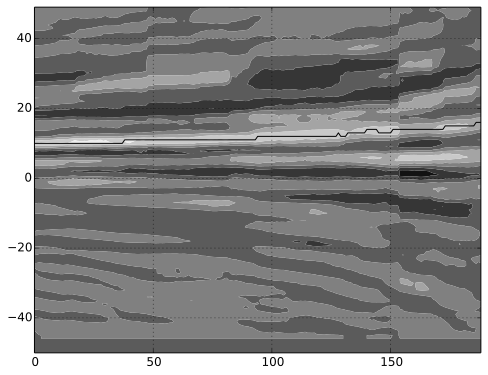
\includegraphics[width=\columnwidth]{selection.pdf}
\caption{Local search strategy for shift selection. Each column of the contour map corresponds to a shift vector. Brighter points indicate higher likelihood. The horizontal axis is time. Starting from a global maximum estimate, hill climbing is performed to update the selected shift while avoiding too much of a deviation from previous values.}
\label{fig:selection}
\end{figure}

Let's now turn to the problem of selecting a change image from the teach step to match against the current replay change image. First, a proper definition of what means for a change image in the replay session to ``correspond'' to an image in the teach session is required. Given a function $\hat{x} = o(t)$ of the robot's position, the \textit{frame correspondence} function $c(t_t, t_r, k)$ can be defined as:
\begin{equation}
c(t_t, t_r, k) = \arg \min_{k' \in [1, n]} {\| o(p(t_t, k')) - o(p(t_r, k)) \|}
\end{equation}

That is, change image $DiVS(w, t_t, k')$ in the range $[DiVS(w, t_t, 1), \dotsc, D(w, t_t, n)]$ ``corresponds'' to current change image $DiVS(w, t_r, k)$ if $k'$ is such that it minimizes the norm of the difference $\| o(p(t_t, k')) - o(p(t_r, k)) \|$ over the range $[1, n]$. Obviously, if $o(t)$ were reliably known at any time, there would be no need for drift estimation in the first place. Therefore what is required is an approximation to $c(t_t, t_r, k)$ that circumvents this requirement.

Several different strategies can be considered. The trivial solution is to correspond change images by index:
\begin{equation}
c_i(t_t, t_r, k) = k
\end{equation}

This may work reasonably well if the robot is driving at the same, constant speed in both the teach and replay steps, and images are sampled at regular intervals (which might depend on implementation factors, such as hardware resources, or how the underlying operating system schedules processes and handles interruptions).

A slightly more elaborate option is to correspond change images by time of acquisition, relative to the start of the session:
\begin{equation}
c_t(t_t, t_r, k) = \arg \min_{k' \in [1, n]} {| (p(t_t, k') - t_t) - (p(t_r, k) - t_r) |}
\end{equation}

This may work better than the previous option when guarantees on regular sampling are poor, but it still assumes a constant speed shared across the two steps.

It's also possible to correspond change images by the distance $x = d(t_0, t)$ traveled since the start of the session:
\begin{equation}
c_d(t_t, t_r, k) = \arg \min_{k' \in [1, n]} {| d(t_t, p(t_t, k')) - d(t_r, p(t_r, k)) |}
\end{equation}

It may seem contradictory to traveled distance on a system ostensibly meant to compensate for inaccuracies in odometry data, but it could work if the odometer is regularly reset -- for example, after the robot passes by key landmarks.

In the implementation and tests detailed later on the distance-based matching strategy is used, but in fact after several tests performed on a range of $10m$ to $20m$, no significant performance difference was found among the three.

Finally, the frame selection function must be defined. The problem is how to ensure that any two subsequent images $(S(p(t, k)), S(p(t, k+1)))$ are different enough to provide useful information, but not too different, as this would increase the noise. A simple solution is again to rely on odometry. Given a function $x = o(t)$ of the robot's position, $p(t, k)$ can be defined such that:
\begin{equation}
p(t, k) = t' \; | \; (k - 1)q \leq o(t') - o(t)
\end{equation}

Where $q$ is the minimal distance traveled by the robot between $p(t, k)$ and $p(t, k+1)$.

\section{Experiments}

A Yamabico robot with a stock web camera mounted to its front was employed in a series of experiments to evaluate the model described above. Its implementation was in the form of the C++ library \textbf{Cight}. Its source code is available on the web under an Open Source license~\cite{HEL14c}. The control system implemented for the robot worked in two modes:

\begin{itemize}
\item Teach: after an optional initial displacement (either an in-place turn or a lateral shift), set off in straight motion at constant speed, stopping after running for $10m$ or receiving an abort command, recording pictures and odometry data along the way;
\item Replay: given a data set of a previous teach session, and after an optional initial displacement to simulate drift, use the Differential Visual Stream method to identify any deviations from the teach path and remain on it.
\end{itemize}

Three environments were used for tests, as illustrated in Figure~\ref{fig:environments}: two outdoors (the front entrance and the parking lot behind research building 3L) and one indoors (the corridor in front of laboratory room 3D402). Tests were performed at different times of the day and varying weather conditions. Linear speed was always set to $0.3m/s$, with pictures and odometry data recorded after every $1.5cm$ on average.

\begin{figure}[h!]
\includegraphics[width=\columnwidth]{environments.pdf}
\caption{Environments used in experiments. (a) View from the front entrance of research building 3L. (b) Parking lot behind the building. (c) Corridor in front of laboratory room 3D402.}
\label{fig:environments}
\end{figure}

\begin{figure}[h!]
\includegraphics[width=\columnwidth]{shift_problem.pdf}
\caption{Changes to apparent position of a far-off landmark relative to the robot's field of view. Starting from a position of perfect alignment between the robot's and landmark's centers (b), an in-place turn of as little as $10^o$ produces a large disparity (b); in contrast, the disparity after a sideways shift as large as half the robot's width is much shorter (c).}
\label{fig:shift_problem}
\end{figure}

\begin{figure}[h!]
\centering
\includegraphics[width=\columnwidth]{changes.pdf}
\caption{Method robustness to lighting and landscape composition changes. Even though visual input for the teach (a) and replay (b) sessions differ substantially, the corresponding change images (c, d) include a number of shared features.}
\label{fig:changes}
\end{figure}

Initially, only teach sessions were recorded. An off-line tool was then used to evaluate whether the method would correctly identify the presence and direction of ``drift'' between pairs of sessions. Parameters for the shift detector were $w = 25$, $d = 50$ and $e = 5$. Table~\ref{tab:entrance_3l_turn} shows results for comparing pairs of teach sessions recorded in front of building 3L. Seven different sessions were recorded: a ``central'' session and six others, that deviated from the original by an in-place turn of $2^o$, $5^o$ or $10^o$, either to the left or right. Table~\ref{tab:car_park_3l_turn} shows results for the same kinds of tests in the parking lot behind 3L, and Table~\ref{tab:corridor_3d_turn}, for the corridor in front of room 3D402.

\begin{table*}[h!]
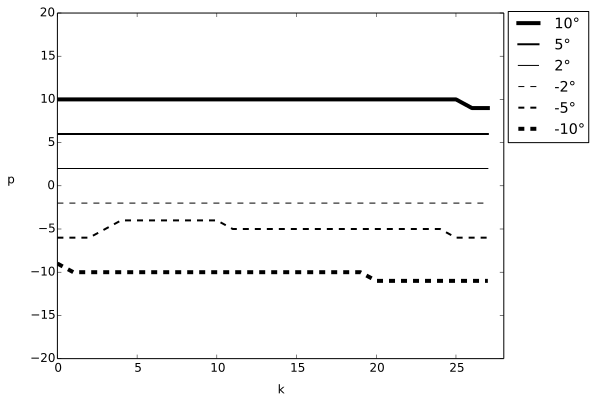
\includegraphics[width=\textwidth]{entrance_3l_turn.pdf}
\caption{Results of comparing a ``central'' teach session with other sessions differing by an initial in-place turn. In each plot, horizontal axis is change image index, and vertical axis is the shift between change images. Positive vertical values indicate a left shift, and negative values, to the right. Brighter regions in the contour map indicate higher shift likelihood: the solid black line running over it indicates the shift value actually selected. Test environment was the entrance of building 3L.}
\label{tab:entrance_3l_turn}
\end{table*}

\clearpage

\begin{table*}[h!]
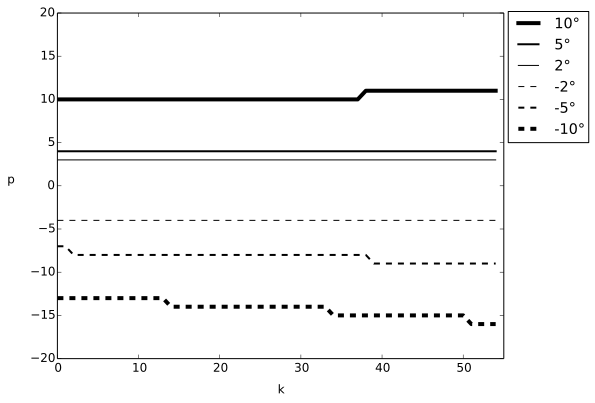
\includegraphics[width=\textwidth]{car_park_3l_turn.pdf}
\caption{Results of comparing a ``central'' teach session with other sessions differing by an initial in-place turn. In each plot, horizontal axis is change image index, and vertical axis is the shift between change images. Positive vertical values indicate a left shift, and negative values, to the right. Brighter regions in the contour map indicate higher shift likelihood: the solid black line running over it indicates the shift value actually selected. Test environment was the parking lot behind building 3L.}
\label{tab:car_park_3l_turn}
\end{table*}

\clearpage

\begin{table*}[h!]
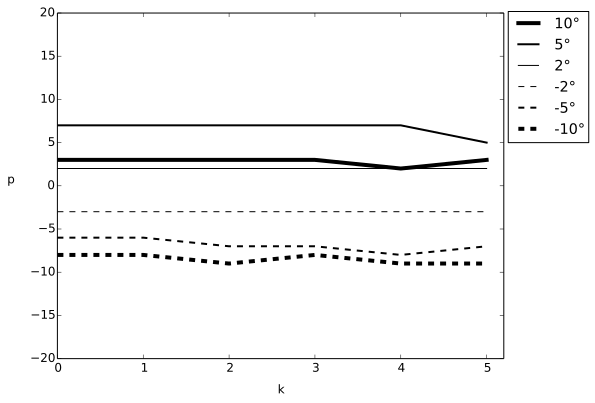
\includegraphics[width=\textwidth]{corridor_3d_turn.pdf}
\caption{Results of comparing a ``central'' teach session with other sessions differing by an initial in-place turn. In each plot, horizontal axis is change image index, and vertical axis is the shift between change images. Positive vertical values indicate a left shift, and negative values, to the right. Brighter regions in the contour map indicate higher shift likelihood: the solid black line running over it indicates the shift value actually selected. Test environment was the parking lot behind building 3L.}
\label{tab:corridor_3d_turn}
\end{table*}

\clearpage

\begin{table*}[h!]
\includegraphics[width=\textwidth]{entrance_3l_shift.pdf}
\caption{Results of comparing a ``central'' teach session with other sessions differing by an initial sideways shift. Sessions were successively recorded in front of building 3L. Sessions recorded under the same initial parameters produce conflicting results.}
\label{tab:entrance_3l_shift}
\end{table*}

\clearpage

\begin{figure}[h!]
\includegraphics[width=\columnwidth]{pedestrian.pdf}
\caption{Resilience against moving elements. Two teach sessions were recorded for the same starting point and heading direction. The first session (a) was recorded in the absence of any moving elements, but in the second (b) a person happened to walk by the robot. Despite this, shift vectors (c) correctly indicate negligible drift was experienced between the sessions.}
\label{fig:pedestrian}
\end{figure}

\begin{figure}[h!]
\centering
\includegraphics[width=\columnwidth]{clutter.pdf}
\caption{Effect of robot directional corrections to the real-time change image. As the robot turns in response to an estimated drift, the (a) initially sparse real-time change image (b) becomes cluttered with changing regions that fell out of alignment with the current sequence.}
\label{fig:clutter}
\end{figure}

Tests with an initial sideways shift were also performed, yielding somewhat less reliable results. As Table~\ref{tab:entrance_3l_shift} shows, successive sessions recorded under the same conditions, with the same amount of shift, would sometimes result in erroneous estimates. Figure~\ref{fig:shift_problem} provides an explanation: compared to in-place turning, sideways shift produces much less disparity in far-off landmarks, which compose the bulk of outdoors landscapes. With much less differences to work on, it's understandable that the system may have problems estimating its exact position.

Some experiments under changing lighting conditions and landscape composition were also performed. Since DiVS shift estimation does not compare individual images, but rather the {\it rates of change} in pairs of image sequences, it is inherently robust to changes that are consistent across whole image sequences, such as overall luminance. It also has a degree of natural resilience to landscape changes, provided they don't substantially affect the rate of change. Figure~\ref{fig:changes} shows an example case.

While most recorded sessions do not depict any moving elements, some unintended records of people walking by the robot were kept for evaluation. Figure~\ref{fig:pedestrian} shows one such case, where despite presence of a walking person in one teach session, but not the other, did not affect the system's correct assessment that there was no significant drift between the sessions.

Replay sessions were also performed. Compared to off-line shift detection between teach sessions, real-time shift detection during replay is complicated by the effects of steering on the change images. As Figure~\ref{fig:clutter} shows, the moment the robot turns in response to a perceived shift, the changing regions of the visual field fall out of alignment with the ongoing sequence, cluttering the change image. To account for this, every time the robot adjusts its heading direction, a new ``time zero'' for calculation of change images is set, causing any images collected during steering to be ignored. Obviously this implies the robot will ``run blind'' for a time, unable to calculate further drift estimates until a while after it has stabilized its heading direction.

The robot's steering algorithm is detailed below:

\begin{enumerate}
\item Load images and odometry from teach step
\item Let the initial robot pose $(x_0, y_0, \theta_0) \gets (0, 0, 0)$
\item Set the robot off in a straight path
\item Let $t_r \gets t$ (i.e. the current time)
\item Let $t_{estimation} \gets t_r$
\item Let $k \gets 0$
\item Let $k \gets k + 1$
\item Wait until $p(t_{estimation}, k+w) \leq t$
\item Let $k' = c_d(t_t, t_r, k)$
\item If $k' = n$, stop the robot and terminate the steering program
\item Let $v_r = v(d, DiVS(w, t_{estimation}, k))$
\item Let $v_t = v(d, DiVS(w, t_t, k'))$
\item Let $shift \gets \arg \max_{i \in [1, d]}{WINC(e, v_t, v_r)}$
\item If $|shift| \leq 1$, go back to step (7)
\item Let $d \gets 1.0$ if $shift < 0$, $d \gets -1.0$ otherwise
\item Adjust the robot's movement so that future pose $(x_{t+\Delta t}, y_{t+\Delta t}, \theta_{t+\Delta t}) \approx (x_t + 0.3, y_t + 0.1d, \theta + d^o)$
\item Let $t_{estimation} \gets t$
\item Wait until $t_{estimation} + \Delta t \leq t$
\item Restore robot movement to a straight path
\item Go back to step (6)
\end{enumerate}

\begin{figure}[h!]
\centering
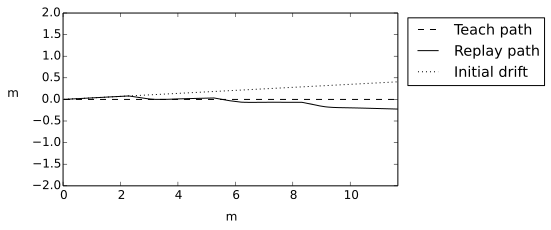
\includegraphics[width=\columnwidth]{car_park_3l_steer_left.pdf}
\caption{Results of replay test performed in the parking lot behind building 3L. Setting off in a straight path after a $2^o$ in-place turn to the left (relative to the heading direction of the teach session), the robot correctly identifies its drifting direction and acts to correct it, but later mistakes its position relative to the teach session path, diverging from it.}
\label{fig:car_park_3l_steer_left}
\end{figure}

\begin{figure}[h!]
\centering
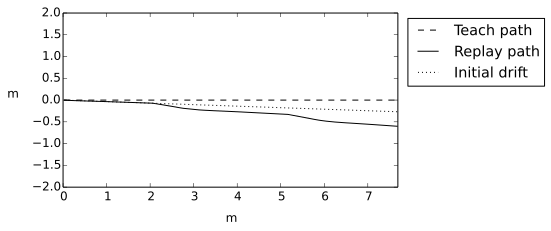
\includegraphics[width=\columnwidth]{car_park_3l_steer_right.pdf}
\caption{Results of replay test performed in the parking lot behind building 3L. Setting off in a straight path after a $2^o$ in-place turn to the right (relative to the heading direction of the teach session), the robot fails to identify its drifting direction and further diverges from the teach session path.}
\label{fig:car_park_3l_steer_right}
\end{figure}

\begin{figure}[h!]
\centering
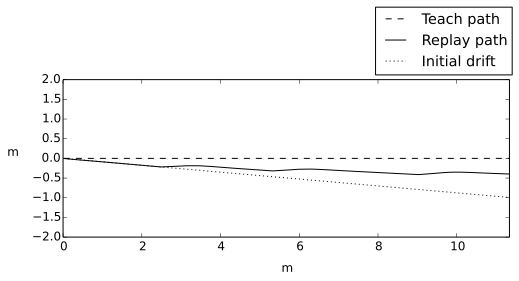
\includegraphics[width=\columnwidth]{entrance_3l_steer_right.pdf}
\caption{Results of replay test performed in front of building 3L. Setting off in a straight path after a $5^o$ in-place turn to the right (relative to the heading direction of the teach session), the robot correctly detects the drift direction and apply successive corrections to its direction, however those were too timid to be effective.}
\label{fig:entrance_3l_steer_right}
\end{figure}

Figure~\ref{fig:car_park_3l_steer_left} shows the results of a typical replay test in the parking lot behind building 3L. Setting off in a straight path after a $2^o$ in-place turn to the left (relative to the heading direction of the teach session), the robot correctly identifies its drifting direction and acts to correct it, but later mistakes its position relative to the teach session path, diverging from it. A second test, where the robot set off after a $2^o$ in-place turn to the right, fared less well: as shown in Figure~\ref{fig:car_park_3l_steer_right}, the robot fails to identify its drifting direction and further diverges from the teach session path.

Another test, performed in front of building 3L, also yielded suboptimal results. As shown in Figure~\ref{fig:entrance_3l_steer_right}, after turning in-place $5^o$ to the right and then setting off, the robot correctly detects the drift direction and apply successive corrections to its direction, however those were too timid to effectively correct the robot's direction.

\section{Conclusion}

Teach-replay is a strategy for autonomous navigation where a robot is first guided along a path, recording data it can use to later retrace it autonomously. This article presented a novel method dubbed \textit{Differential Visual Stream} (DiVS) for appearance-based visual navigation under teach-replay. DiVS can be used to detected shifts between image sequences. This in turn can be used to estimate the robot's drift from the teach path during replay. The method is robust to changes in lighting and landscape composition, as well as the presence of moving elements. It is also suitable for use both indoors and outdoors.

Currently DiVS's main limitation is that it provides \textit{shift} estimates (i.e. differences in landscape perception) but what is really required are \textit{drift} estimates (i.e. differences in robot pose). At this time a control algorithm was used that essentially tries to guess pose drift from image shift, with suboptimal results. Also the inability to use images acquired while the robot is steering poses a serious limitation to reaction times. Both issues must be subjected to further research.

\footnotesize

\bibliographystyle{IEEEtran}
\bibliography{references}

\normalsize

\end{document}
